%$Id$
\documentclass[conference, compsoc]{IEEEtran}
\usepackage{fontspec}
%\usepackage{amsmath,amssymb,amsthm,supertabular,booktabs,rotating,semantic,subfigure,multirow,colortbl}
\usepackage{graphicx, url}
\usepackage[colorlinks=true,linkcolor=black,anchorcolor=black,citecolor=black,urlcolor=black,bookmarks=false,pdfstartview=FitH]{hyperref}
\usepackage{algorithmic,algorithm}
\usepackage{xunicode}
\usepackage{colortbl}
\usepackage{xltxtra}
\defaultfontfeatures{Mapping=tex-text}
\setmainfont{Times New Roman}
\begin{document}

\bibliographystyle{IEEEtran}
 
\title{Understanding software quality evolution using signifier frequency extraction}
\author{
Neil A. Ernst\\Dept. of Computer Science\\University of Toronto\\nernst@cs.toronto.edu \and
John Mylopoulos\\Dept. of Computer Science\\University of Toronto\\jm@cs.toronto.edu }

\maketitle

\begin{abstract}
This paper describes a software repository mining technique we call signifier extraction. Signifiers are keywords about software quality that we generate using Wordnet and the ISO quality taxonomy. Using corpora created from eight Gnome projects -- their mailing lists, subversion comments, and bug comments -- we search for the signifiers over three month, quarterly intervals. The occurrence of our signifiers forms an evolutionary pattern that we analyze statistically and historically. We show that it is possible to reconstruct the historical evolution of software qualities as responses to external forcings, such as release cycles and usability audits. %[numbers?]
\end{abstract}
\vspace{-2mm}
\section{Introduction}\label{sect:introduction}%Aim
\vspace{-2mm}
\begin{quote}[My impression] is of a large project in a state of marginal returns, in which a larger and larger part of the effort goes to maintenance. -- Andy Wingo, Gnome developer, June 2008.\footnote{http://wingolog.org/archives/2008/06/07/gnome-in-the-age-of-decadence}\end{quote}
	This quote, from a developer in the Gnome ecosystem, captures some of what this paper tries to explore. Is it the case that as projects mature the focus and effort of the developers must turn to maintenance tasks\cite{Swanson1976}? %Certainly Lehman's conclusion~\cite{lehman_software_2006} is that this is the case (viz. Lehman's 7th `law'). 
This paper takes up the question as to whether this can be empirically demonstrated. To test this notion, we begin with a few assumptions. The first is that there is some sort of signal we can capture that will signify that `maintenance' is being done. One approach is to scan code for maintenance activity, using, for example, formal concept analysis~\cite{breu06msr}. Our approach, by contrast, is focused on the conversations developers have (with each other, or with `users'). To identify when `effort goes to maintenance', we further assume that discussion about software quality is an effort spent on maintenance, and moreover, that discussions about maintenance often involve a set of common terms, which we call signifiers. We define these using the ISO 9126-1 software quality model \cite{iso9126} as a starting point. 
	
Section \ref{sec:Method} describes how we derive these signifiers and how we built our corpora and toolset for extracting the signifiers. We then present our observations and a discussion about significance in Section \ref{sec:observations}. Finally, we examine some threats to our approach and discuss related work. 

\noindent\textbf{Related Work}
Part of our efforts with this project is to reconstruct a history of the software product's evolution, a notion we first discussed in \cite{Ernst07icsm}. That idea is derived from, in part, work on narratives of software systems shown in academic work like \cite{Anton2001} or more general-purpose works like \cite{waldo93}. Software mining of the type we do, a type of reverse formal concept analysis, is less common. Similarities exist with approaches that begin with structured taxonomies, as with the Hismo software ontology \cite{Girba2006}.
	
\vspace{-2mm}
\section{Methodology}
\vspace{-2mm}
\label{sec:Method}
Our dataset is a selection of eight Gnome projects (listed on the Gnome wiki), shown in Table \ref{tbl:projects}\footnote{Source code, processed data, and related discussions are available at \url{http://neilernst.net/archives/tag/msr/}.}. The projects were selected to represent a variety of lifespans (from 18 months to 11 years) and code sizes. For each project we extracted text-based datasets: that project's mailing list (except for Ekiga and Empathy which have no apparent mailing list); that project's subversion logs; and finally, the bug comments for the project. We extracted the date, text (which we term an `event'), and source, and placed this information into a MySQL database.

%\subsection{Signifier extraction}
\begin{table}
	\caption{Selected Gnome ecosystem products}
	\centering
	\label{tbl:projects}
\begin{tabular}{|c|c|c|c|}
\hline
\rowcolor[gray]{.9} 
\textbf{Product} & \textbf{Language} & \textbf{Size} \emph{(Kloc)} & \textbf{Age} \emph{(years)} \\
\hline
\hline 
Evolution & C & 313 & 10.75\\ \hline
Nautilus & C & 108 & 10.75  \\ \hline
Metacity & C & 66 & 7.5  \\ \hline
Ekiga & C++ & 54 & 7  \\ \hline
Totem & C & 49 & 6.33  \\ \hline
Deskbar & Python/Sh & 21 & 3.2  \\ \hline
Evince & C & 66 & 9.75\\ \hline
Empathy &C & 55 & 1.5\\ 
\hline
\end{tabular}
\end{table}

In semiotics, Peirce drew a distinction drawn between signifier, signified, and sign~\cite{atkin2006}. In this work, we make use of signifiers -- words like `usability' and `usable' -- to capture the occurrence in our corpora of the signified -- in this example, the concept `usability'. We extract our signified, concept words from the ISO 9126 quality model~\cite{iso9126}. There is some debate about the significance and importance of the terms in this model. However, it is ``an international standard and thus provides an internationally accepted terminology for software quality~\cite[p. 58]{Boegh2008},'' which is sufficient for the purposes of this research. The model is used to refer to both external and internal views of quality (for example, bugs filed by users would be external qualities, whereas an email discussion of features to come would be internal). We generate the signifiers from Wordnet~\cite{Fellbaum1998}, an English-language `lexical database' that contains semantic relations between words, including meronymy and synonymy. We extract words using the procedure defined in \ref{alg1}. The only deviation we made was to add the term `performance' to the synonyms for `efficiency', since this seems like a common synonym in this domain.% (Wordnet is not domain-specific). %A complete list is available online (see Section \ref{appendix}). %This factor shows up in the higher error rates, particulary for two word terms like time behaviour.

\renewcommand{\algorithmiccomment}[1]{// #1}
\begin{algorithm}[H]
\caption{Defining signified terms extensionally}
  \label{alg1}
\begin{algorithmic}
	\REQUIRE $T$, the set of top-level terms in ISO9126-1
  	\FORALL{$t \in T$}
	\STATE $S \leftarrow \emptyset $
    %\STATE define $t$ as a wordnet noun
	\STATE identify synset of $t$ (synonyms)%  from Wordnet
	\STATE $S \leftarrow S +$ synset
	\STATE identify direct hypernyms of $t$ (specializations)% from Wordnet
	\STATE $S \leftarrow S +$ hypernyms %is-a
	\STATE identify meronyms of $t$ (components)% from ISO9126
	\STATE $S \leftarrow S +$ meronyms %part-of
	\STATE identify related forms of $t$ (stemmed)% from Wordnet
	\STATE $S \leftarrow S +$ related forms
	\FORALL {$s \in S$}
		\STATE query corpora for $s$
		\COMMENT ignore case
	\ENDFOR
  \ENDFOR
\RETURN $E$, the set of unique `events' per $t$

\end{algorithmic}
\end{algorithm}
Note, we do not currently look for common misspellings or other languages (the primary language is English, at any rate). This algorithm gives us a linguistic `bubble' which we use to extensionally define the signified term, as shown in Fig. \ref{fig:syngraph}. An event is any row in the table which contains at least one term in the bubble (i.e., don't double count). Our MySQL queries produced a set of unique events (e.g., a subversion commit message), averaged over quarters of years, and the associated time and project. From this we conducted our observations and statistical tests.

\begin{figure}[b]
\centering
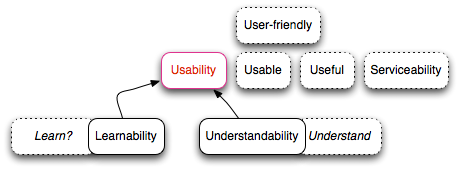
\includegraphics[width=0.4\textwidth]{synonym-graph.pdf}
\caption{An extensional definition of usability, showing in dashed lines those concepts outside our signifier `bubble'.}
\label{fig:syngraph}
\end{figure}

\section{Observations}
\label{sec:observations}
Fig. \ref{fig:n-use-line} and Fig. \ref{fig:ev-eff-line} shows two examples of our queries. The red line connects a number of events for that particular quarter. For example, in the third quarter of 2000, there were approximately 80 normalized events in the Evolution project for Efficiency. We normalize the extracted event numbers to remove the effect of changes in mailing list volume or commit log activity. The calculation takes the extracted events, divides by the total events, and multiplies by 1000. The black line is a linear regression, and the dashed vertical lines represent Gnome project milestones, with which most of the projects we study are synchronized.

\begin{figure*}[ht]
\begin{minipage}[]{0.5\textwidth}
\centering
\includegraphics[width=\textwidth]{figures/Nautilus-Usabilityline.png} 
\label{fig:n-use-line}
\caption{Product: Nautilus, Quality: Usability}
\end{minipage}%
%\hspace{0.2cm}
\begin{minipage}[]{0.5\textwidth}
\centering
\includegraphics[width=\textwidth]{figures/Evolution-Efficiencyline.png}
\label{fig:ev-eff-line}
\caption{Product: Evolution, Quality: Efficiency}
\end{minipage}
\end{figure*}

\vspace{-2mm}
\subsection{Discussion}
\vspace{-2mm}

We include a linear regression of the number of occurrences against the date. The equation of the regression line shows the average value of the number of occurrences as the date increases. A linear relationship may not be a good model of the actual pattern. For example, the number of occurrences may be changing in response to some other variable, such as co-ordinated release dates, which we show in Fig. \ref{fig:ev-eff-line} as vertical gray lines, and which we discuss below; or by things such as developer illness. Due to space constraints, Table \ref{tbl:summary} lists only the two longest-lived projects, and $r^2$  -- squared correlation value -- and slope (trend) values for each quality. We ended up with largely conflicting numbers. 

\begin{table}
	\caption{Selected summary statistics, normalized}
	\centering
	\label{tbl:summary}
\begin{tabular}{|c|c|c|}
\hline
\rowcolor[gray]{.9} 
File-Keyword &  $r^2$ &  slope \\ \hline
Evolution-Efficiency & 0.07 & -0.38 \\
Evolution-Portability & 0.12 & -0.36 \\
Evolution-Maintainability & 0.05 & -0.27 \\
Evolution-Reliability & 0.08 & -0.29 \\
Evolution-Functionality & 0.05 & 0.92 \\
Evolution-Usability & 0.12 & -1.38 \\
Nautilus-Efficiency & 0.19 & -4.77 \\
Nautilus-Portability & 0.11 & -0.51 \\
Nautilus-Maintainability & 0.37 & -1.49 \\
Nautilus-Reliability & 0.38 & -1.00 \\
Nautilus-Functionality & 0.26 & -4.22 \\
Nautilus-Usability & 0.23 & -7.96 \\
% Totem-Efficiency & 0.03 & -1.86 \\
% Totem-Portability & 0.06 & -0.35 \\
% Totem-Maintainability & 0.00 & 0.02 \\
% Totem-Reliability & 0.02 & 0.19 \\
% Totem-Functionality & 0.16 & -1.87 \\
% Totem-Usability & 0.33 & -1.97 \\
\hline
\end{tabular}
\end{table}

We therefore sought alternative explanations for the patterns seen in our data. We first investigated smaller event windows, based around the period between major Gnome releases; secondly, we used the identified peaks in the data to explore possible causative events. We chose the Efficiency (performance) and Usability qualities for further exploration.

\begin{table}
	\caption{Normalized statistics for release window technique}
	\centering
	\label{tbl:windows}
\begin{tabular}{|c|c|c|c|c|}
\hline
\rowcolor[gray]{.9} 
File-Keyword & Release \# & $r^2$ & slope & N\\ \hline
Evolution-Eff. & 1.4 & 0.23 & -0.67 & 20 \\
 & 2.24 & 0.62 & -1.13 & 7\\ \hline
Evolution-Usab. & 1.4 & 0.01 & -0.11 & 32\\
 & 2.24 & 0.04 & -0.52 & 10 \\ \hline
Nautilus-Eff. & 1.4 & 0.04 & 0.52 & 25 \\
 & 2.24 & 0.75 & -6.64 & 4 \\ \hline
Nautilus-Usability & 1.4 & 0.14 & 0.79 & 31\\
 & 2.24 & 0.01 & 0.97 & 14\\

\hline
\end{tabular}
\end{table}

\noindent\textbf{Using release windows} -- It's possible that the peak event occurrences are more strongly correlated with the time period prior to a major release, that is, cyclical. In the left side of Fig. \ref{naut-use-line}, there seems to be a major upward trend prior to the release of Gnome 2.0, a co-ordinated release. We defined release windows to investigate whether there was higher correlation between number of events and time for selected projects and keywords. Table \ref{tbl:windows} shows our results for selected products and releases. For some release dates, we see a high degree of correlation; however, the pattern is not seen in other dates, suggesting the results are not predictive. 

\noindent\textbf{Analysis of key peaks in selected graphs} - The final explanation we explore is that the data are independent of software age, or release cycle, and are instead responding to external events. For example, there may be a usability audit, or a review by a major news source of the performance of the project, etc. Accordingly, we chose two products -- Evolution, a calendar and email application, and Nautilus, a web browser and file manager, for more detailed analysis. We examined Efficency (including performance) and Usability events for each, choosing a major peak for each to attempt some historical analysis. Our approach allows us to target our historical analysis more precisely. We looked at the peaks

%TODO Expand this. Use a series of checks, starting with Gnome release/project release date, mailing list threads, source code, wider events (Sept 11)
\noindent\textbf{Accuracy} -- We performed error analysis on our results. What we wanted to verify was the percentage of terms retrieved that were unrelated to a software quality. For example, we encountered some mail messages from individuals whose email signature included the words ``Usability Engineer''. If the body of the message wasn't obviously about usability, we coded this as a false-positive. We did not assess the rate of false-negatives (as mentioned above). Our tests involved randomly selecting messages from the corpora and coding them as relevant or irrelevant. We assessed 100 events per signified term to generate our rates. Table \ref{tbl:error} presents the results of this test. In general, false-positives averaged 23\% of events.

\begin{table}
	\caption{False positive rates}
	\centering
	\label{tbl:error}
\begin{tabular}{|c|c|}
\hline
Signified quality & F.P. Rate  \\
\hline
\hline
Usability & 0.19\\ \hline
Portability & 0.29\\ \hline
Maintainability & 0.13\\ \hline
Reliability & 0.23\\ \hline
Functionality & 0.14 \\ \hline
Efficiency & 0.41\\ \hline
\hline
\end{tabular}
\end{table}

\noindent\textbf{Threats to validity} -- The main threat to construct validity is that our signifiers omit relevant terms or phrases., e.g., ``can't find the submit button" vs. ``usability". Furthermore, we may want to use the term `User friendly' in relation to `usability'. A more domain-specific taxonomy would be useful. Our data originated from open-source projects, less than ten years old, from the Gnome ecosystem, primarily using \texttt{C} code, so these are threats to external validity.

\vspace{-2mm}
\section{Conclusions and future work}
\vspace{-2mm}
In the introduction we mentioned our hypothesis that software qualities ought to be of more interest to a community as the project matures. Our data provided mixed evidence for this hypothesis. We found some positive correlation between age and qualities, but in general, the correlations were too weak to draw strong conclusions this way. Instead, we explained a few of the more significant events by examining the possible external causes. These conclusions are qualitative, but draw on historiographical techniques for support.

Our ultimate goal is to be able to extract, from available sources, a list of requirements for a project, so that we can trace not just the `physical' changes in the codebase, but also the evolving features and goals inherent in a project. We plan to continue our experiments with repository mining with this in mind. In all likelihood, we will need to expand both our taxonomy (to be more software development specific) and our data sources (including source code comments or wiki pages, for example).

A secondary direction is related to the social aspect of software development. Each event in our database is initiated by somebody and involves other contributors. It would be interesting to see whether certain individuals are responsible solely for particular software qualities. Hindle et al., in \cite{hindle09icpc}, showed that such information contains a high degree of signal.

% \vspace{-2mm}
% \section{Appendix and acknowledgements}
% \vspace{-2mm}
% \label{appendix}

%Thanks to the comments of the software engineering group at the University of Toronto.
\begin{footnotesize}
	\vspace{-2mm}
	
\bibliography{msr}
\vspace{-2mm}
\end{footnotesize}
\end{document}



% I suspect the underlying problem you are having is how
% to cope with requirements churn. From Mary Poppendieck's
% book "Implementing Lean Software Development" there's this
% very valuable tip:
% 
% "If you have requirements churn, you are specifying too
% early".